\documentclass[11pt,aspectratio=43]{beamer}
\usepackage[utf8]{inputenc}
\usepackage{amsmath, amsfonts, amssymb, amsthm}
\usepackage[T1]{fontenc}
\usepackage{lmodern}
\usepackage{xcolor}
\usepackage{setspace}
\usepackage{booktabs}
\usepackage{multirow}
\usepackage{graphicx}
\usepackage{tikz}
% \usetikzlibrary{decorations}
\usetikzlibrary{decorations.pathreplacing}
\usepackage{ulem}
\usepackage{hyperref}
% \hypersetup{colorlinks=true,allcolors=blue}
\usepackage{booktabs}
\usepackage{babel}
\usepackage{makecell}
\usepackage[para,online,flushleft]{threeparttable}
\usepackage{pdfpages}
\usepackage{tcolorbox}
\usepackage{bm}
\usepackage{appendixnumberbeamer}
\usepackage{natbib}
\usepackage{caption}
\captionsetup[figure]{labelformat=empty}% redefines the caption setup of the figures environment in the beamer class.
\usetheme[compress]{Boadilla}
\usecolortheme{default}
\useoutertheme{miniframes}
\usefonttheme[onlymath]{serif}

\newcommand{\jump}[2]{\hyperlink{#1}{\beamerbutton{#2}}}
\newcommand{\orange}[1]{\textcolor{orange}{#1}}
\newcommand{\red}[1]{\textcolor{red}{#1}}

\setbeamertemplate{itemize item}{\raisebox{0.1em}{\scalebox{0.7}{$\blacksquare$}}}
\setbeamertemplate{itemize subitem}[circle]
\setbeamertemplate{itemize subsubitem}{--}
\setbeamercolor{itemize item}{fg=black}
\setbeamercolor{itemize subitem}{fg=black}
\setbeamercolor{itemize subsubitem}{fg=black}
\setbeamercolor{item projected}{bg=darkgray,fg=white}
\definecolor{blue}{rgb}{0.2, 0.2, 0.7}
\setbeamercolor{alerted text}{fg=blue}
\setbeamertemplate{enumerate items}[circle]


\setbeamertemplate{headline}{}

%==========================================
\let\olditemize=\itemize
\let\endolditemize=\enditemize
\renewenvironment{itemize}{\olditemize \itemsep1em}{\endolditemize}
\let\oldenumerate=\enumerate
\let\endoldenumerate=\endenumerate
\renewenvironment{enumerate}{\oldenumerate \itemsep1em}{ \endoldenumerate}

\DeclareMathOperator*{\argmax}{\arg\!\max}
\DeclareMathOperator*{\E}{\mathbb{E}}
\DeclareMathOperator*{\var}{\rm Var}
\DeclareMathOperator*{\cov}{\rm Cov}

\theoremstyle{definition}
\newtheorem{assume}{Assumption}
\newtheorem{lem}{Lemma}
\newtheorem{proposition}{Proposition}
\newtheorem{thm}{Theorem}
\newtheorem{corol}{Corollary}

\begin{document}
    \title[Lecture 1]{Lecture 1: Introduction \\ Course and Macroeconomics}
    \author[Hui-Jun Chen]{Hui-Jun Chen}
    \institute[OSU]{The Ohio State University}
    % \date{\today}
    \date{\today}
    \setbeamertemplate{navigation symbols}{}
    \setstretch{1.2}

%-------------------------------------------------------
{
%	\usebackgroundtemplate{\includegraphics[width=1\paperwidth]{../EveningSky_cropped_edit43_bright.jpg}}
    \begin{frame}
% \vspace{3em}
        \centering
%		{\footnotesize 	ECON 4002 Intermediate Macroeconomic Theory}
        \maketitle
% \vspace{-1.5em}
% \centering
% \includegraphics[width=0.55\linewidth]{Pictures/houses.jpeg}


    \end{frame}
}

% -------------------------------------------
\setbeamertemplate{headline}
{
\setbeamercolor{section in head/foot}{fg=black, bg=white}
\vskip1em \tiny \insertsectionnavigationhorizontal{1\paperwidth}{\hspace{0.6\paperwidth}}{}
}
%------------------------------------------

\section{Course Plan}
\label{sec:Course_Plan}

\begin{frame}{Your Instructor}
\label{slide:Your_Instructor}
    \begin{itemize}
        \item My name is \alert{Hui-Jun Chen}, you can call me HJ for convenience.
        \item I am interested in \alert{housing}, \alert{used capital market}, and their macroeconomics implications.
        \item In my leisure time, I also like to investigate the \alert{Linux} system.
        \item Contact Info:
        \begin{itemize}
            \item Email: \href{chen.9260@buckeyemail.osu.edu}{chen.9260@buckeyemail.osu.edu}.
            \item Website: \href{https://huijunchen9260.github.io/}{https://huijunchen9260.github.io}
        \end{itemize}
    \end{itemize}
\end{frame}



\begin{frame}{Basics}
\label{slide:Basics}
    \begin{itemize}
        \item Class Meetings: Tuesday and Thursday, 11:40 AM to 1:15 PM
        \item Zoom Info:
        \begin{itemize}
            \item Meeting ID: 951 7226 1996
            \item Password: 946301
            \item \href{https://tinyurl.com/2s4hr365}{Direct Link}:
                    \href{https://tinyurl.com/2s4hr365}{https://tinyurl.com/2s4hr365}
                    (Shorten by tinyurl)
        \end{itemize}
        \item Documents and lecture recordings will be posted on \href{https://tinyurl.com/yfpt8nsn}{Course Website}:
        \begin{itemize}
            \item Direct Link: \href{https://tinyurl.com/yfpt8nsn}{https://tinyurl.com/yfpt8nsn}
        \end{itemize}
        \item Announcement, quiz and exams will be made via \href{https://osu.instructure.com/courses/121985}{Carmen}
        \begin{itemize}
            \item Direct Link: \href{https://osu.instructure.com/courses/121985}{https://osu.instructure.com/courses/121985}
        \end{itemize}
    \end{itemize}
\end{frame}

\begin{frame}{Basics (Cont.)}
\label{slide:Basics__Cont__}
    \begin{itemize}
        \item To get email reply, you \textbf{must} satisfy two conditions below:
        \begin{enumerate}
            \item \alert{DO \textbf{NOT} SEND TO CARMEN EMAIL}
            \item \alert{Use \texttt{[E4002.01]} at the beginning of your subject title}
            \begin{itemize}
                \item example title: \texttt{[E4002.01] Question regarding Extra credit}
            \end{itemize}
        \end{enumerate}
        \item I will reply your email within \textit{2 business day}.
        \item Office hour: One hour before the lecture
        \begin{itemize}
            \item Tuesday and Thursday, 10:40AM - 11:40AM, on \href{https://osu.zoom.us/j/95172261996?pwd=bHVuRlU5dHlmSUx5STcycDBkOVdpZz09}{Zoom Link}
            \item Please tell me if you plan on coming!
        \end{itemize}
    \end{itemize}
\end{frame}

\begin{frame}{Expectation}
\label{slide:Expectation}
    \begin{columns}
        \begin{column}{0.6\textwidth}
            \begin{itemize}
                \item \textbf{Attendance}: recommended but not required
                \item \textbf{Participation}: can ask question anytime during the lecture
                \begin{itemize}
                    \item Just interrupt me by asking. Can check zoom chat but might not very often.
                \end{itemize}
                \item \textbf{Prerequisites}: \alert{Principle of Economics}
                        (ECON 2001 \& 2002),
                        Basic Algebra
                \item \textbf{Calculus}: better to know in advance, but will learn via video series \alert{\href{https://www.youtube.com/watch?v=WUvTyaaNkzM&list=PLZHQObOWTQDMsr9K-rj53DwVRMYO3t5Yr}{The Essence of Calculus}}
            \end{itemize}
        \end{column}
        \begin{column}{0.4\textwidth}
            \begin{figure}
                
\includegraphics[width=\textwidth]{./figures/Williamson.jpg}
                \caption{Recommended but not required textbook}
            \end{figure}
        \end{column}
    \end{columns}
\end{frame}

\begin{frame}{Quiz, Exam and Homework}
\label{slide:Exam__Quiz_and_Homework}
    \begin{itemize}
        \item \textbf{Quiz}: Weekly by watching \alert{\href{https://www.youtube.com/watch?v=WUvTyaaNkzM&list=PLZHQObOWTQDMsr9K-rj53DwVRMYO3t5Yr}{The Essence of Calculus}} ($ 20\% $)
        \begin{itemize}
            \item \alert{unlimited} time and trials w/ a week, meant to encourage!
            \item Will drop 1 lowest quiz between Ch. 1-9.
        \end{itemize}
        \item \textbf{Exam}: Midterm and Cumulative Final, $ 30\% $ each
            \begin{itemize}
                \item Midterm: \alert{June 23Th, 2022}
                \item Final: \alert{August 2nd, 2022}
            \end{itemize}
        \item \textbf{Homework}: on \alert{\href{https://osu.instructure.com/courses/121985}{Carmen}} ($20\%$)
        \begin{itemize}
            \item A good representation for exam
            \item step-by-step guidance on calculation
        \end{itemize}
        \item Schedule and Deadline: see syllabus
    \end{itemize}
\end{frame}



\begin{frame}{Course Plan}
\label{slide:Course_Plan}
\begin{itemize}
    \item \textbf{Module 1}: Measurement (Week 1)
    \begin{itemize}
        \item stylized facts about Economics growth and business cycle
    \end{itemize}
    \item \textbf{Module 2}: One-period (\alert{static}) model (Week 2-6)
    \begin{itemize}
        \item micro foundation: consumers and firms
        \item macro implication: equilibrium, efficiency, resource allocation w/ data
    \end{itemize}
    \item \textbf{Module 3}: Two-period (\alert{dynamic}) model (Week 8-12)
    \begin{itemize}
        \item module 2 $ + $ time: \alert{intertemporal substitution}
    \end{itemize}
\end{itemize}
\end{frame}

\section{Methodology of Macro}
\label{sec:Methodology_of_Macro}

\begin{frame}{What is Macro?}
\label{slide:What_is_Macro_}
    \begin{itemize}
        \item ``\alert{macro is a method}''
        \item Models (theory) $ + $ Data (empiric) $ = $ explanation to macro events
        \begin{itemize}
            \item w/o models: only \alert{correlation}
            \item w/o data: only \alert{imagination}
            \item \alert{Friedman's critique}: models are judged by \alert{prediction power}
        \end{itemize}
        \item Macro events in this class: \alert{long-run growth} and \alert{business cycle}
        \begin{itemize}
            \item what drives long-run trend in US GDP?
            \item what causes the fluctuation in GDP growth?
        \end{itemize}
        \item Macro connects with micro
        \begin{itemize}
            \item individual decisions (micro) $ \Rightarrow  $ aggregates (macro)
        \end{itemize}
    \end{itemize}
\end{frame}

\begin{frame}{Data Example: GDP per capita}
\label{slide:Data_Example__GDP}
    \begin{itemize}
        \item \textbf{Definition}: Gross Domestic Product \alert{per individual}
        \begin{itemize}
            \item quantity produced of \alert{goods $ + $ services} w/i country \alert{border} at given \alert{period of time}
        \end{itemize}
        \item \textbf{Measurement}: $ 3 $ possible approaches
        \begin{itemize}
            \item Product, Expenditure, Income
            \item Source: National Income and Product Accounts (NIPA)
        \end{itemize}
        \item \textbf{Analysis}: separation data into \alert{trend} and \alert{business cyclie}
    \end{itemize}
\end{frame}

\begin{frame}{Real GDP per capita, 1900-2014}
\label{slide:Real_GDP_per_capita__1900_2020}
    \begin{columns}
        \begin{column}{0.5\textwidth}
            \begin{figure}
                \caption{Figure 1.1: Per Capita Real GDP (in 2009 dollars) for the United States, 1900–2014 \\ \alert{$Y$}}
                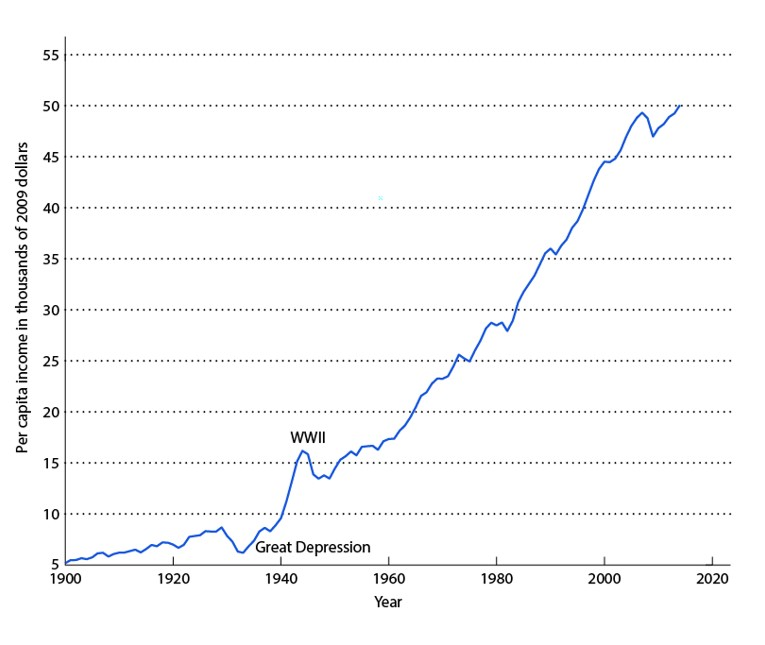
\includegraphics[width=\textwidth]{./figures/Figure1_1.jpg}
            \end{figure}
        \end{column}
        \begin{column}{0.5\textwidth}
            \begin{figure}
                \caption{Figure 1.3: Natural log of Per Capita Real GDP and trend, 1900–2014 \\ \alert{$y = \ln(Y), trend = HPFilter(y)$}}
                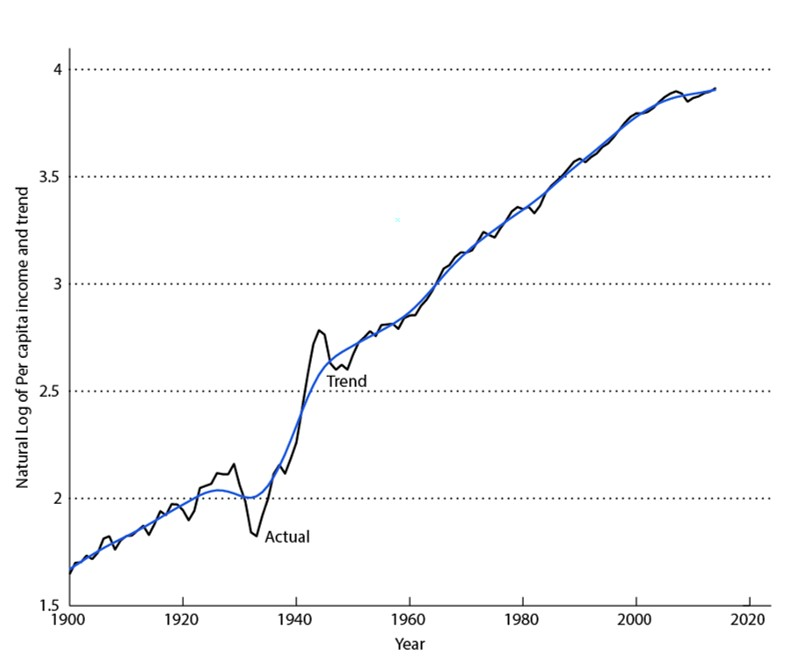
\includegraphics[width=\textwidth]{./figures/Figure1_3.jpg}
            \end{figure}
        \end{column}
    \end{columns}
\end{frame}

\begin{frame}{Business Cycle: Deviation from Trend}
\label{slide:Business_Cycle__Deviation_from_Trend}
    \begin{columns}
        \begin{column}{0.5\textwidth}
            \begin{figure}
                \caption{Figure 1.4 Percentage Deviation from Trend in Per Capita Real GDP \\ \alert{actual - trend}}
                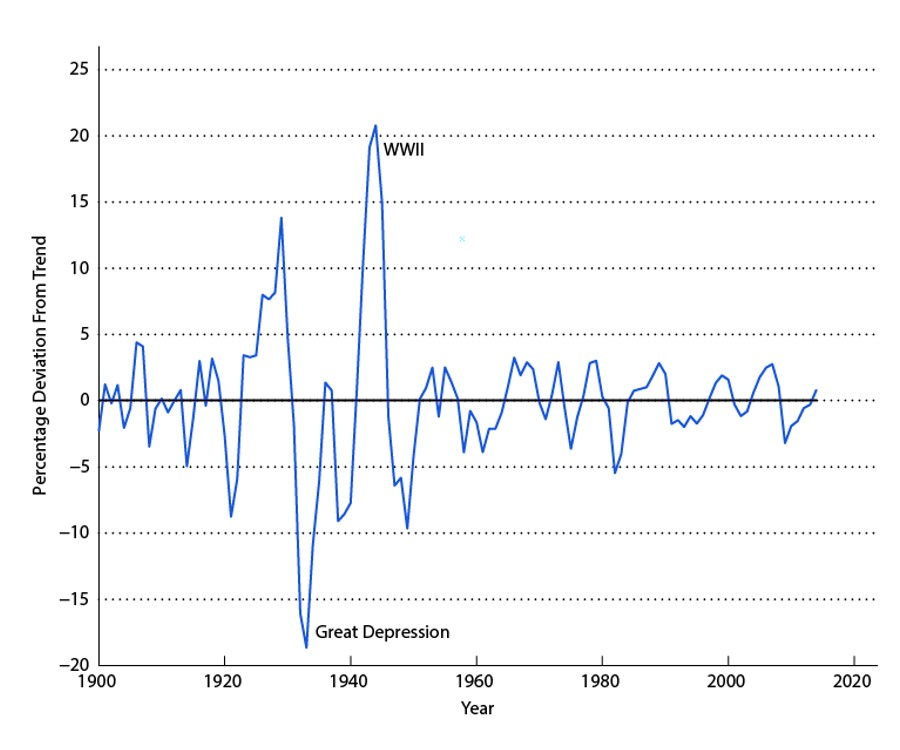
\includegraphics[width=\textwidth]{./figures/Figure1_4.jpg}
            \end{figure}
        \end{column}
        \begin{column}{0.5\textwidth}
            \begin{figure}
                \caption{Figure 1.13 Percentage Deviation From Trend in Real GDP \\ \alert{same transform as 1.1, 1.3, 1.4, not per capita} }
                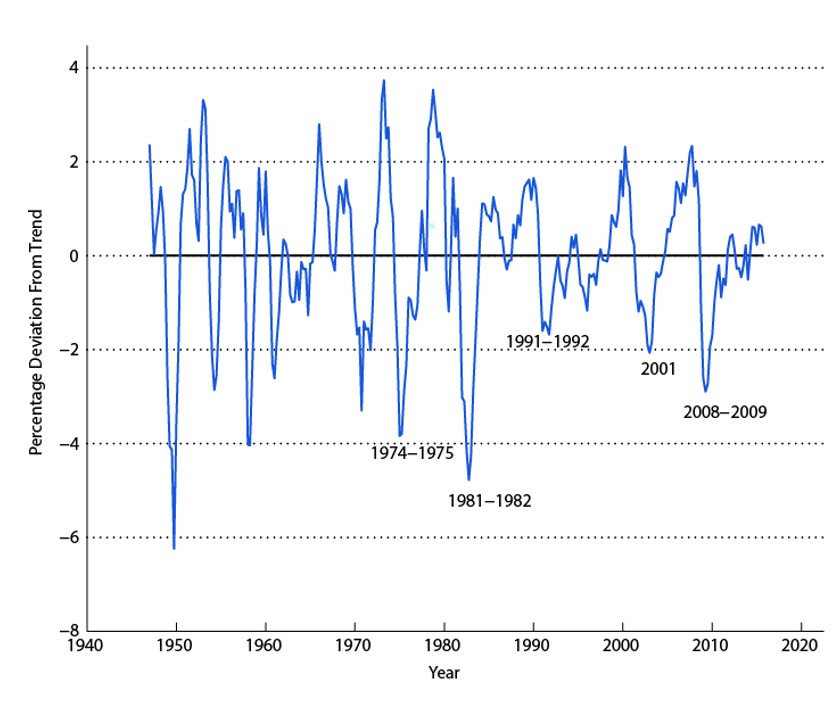
\includegraphics[width=\textwidth]{./figures/Figure1_13.jpg}
            \end{figure}
        \end{column}
    \end{columns}
\end{frame}

\begin{frame}{Using Macro Model to Understand Data}
\label{slide:Using_Macro_Model_to_Understand_Data}
    \begin{itemize}
        \item Economics is a \alert{scientific pursuit} involving the formulation and \alert{refinement of theories} that can help us better understand \alert{how economies work} and \alert{how they can be improved}
        \item \textbf{Data}: \alert{how economies work}, e.g. GDP example
        \item \textbf{Theory}: cannot do experiment, only way for \alert{scientific pursuit}
        \item \textbf{Policy}: understand \alert{how economies can be improved} by \alert{policies}
    \end{itemize}
\end{frame}

\begin{frame}{Structure of Macro Model: $ 4 $ elements}
\label{slide:Structure_of_Macro_Model____4___elements}
\begin{enumerate}
    \item \textbf{agent}: who is involved?
    \begin{itemize}
        \item e.g. consumers, firms, governments, etc.
    \end{itemize}
    \item \textbf{preferences}: how and what is consumed/valued/invested?
    \begin{itemize}
        \item e.g. consumers' utility function on goods
    \end{itemize}
    \item \textbf{resources}: availability and distribution
    \begin{itemize}
        \item e.g. Wealth, time, talents, natural resources
    \end{itemize}
    \item \textbf{technology}: objective limitation at given period of time
    \begin{itemize}
        \item firms' production, market structure
    \end{itemize}
\end{enumerate}
\end{frame}

\begin{frame}{Analysis on Macro Model: $ 3 $ steps}
\label{slide:Analysis_on_Macro_Model____3___steps}
    \begin{enumerate}
        \item \textbf{Equilibrium}: how do all the forces balanced?
        \begin{itemize}
            \item e.g. competitive equilibrium
        \end{itemize}
        \item \textbf{Assessment}: what's model prediction, and how different from data?
        \begin{itemize}
            \item relationship between consumption and output
        \end{itemize}
        \item \textbf{Refinement}: how do changes in model alter its prediction?
        \begin{itemize}
            \item different technology, one-period $ \rightarrow  $ two-period
        \end{itemize}
    \end{enumerate}
\end{frame}



\begin{frame}{Just Micro?}
\label{slide:Just_Micro_}
    \alert{Yes!} Macro models need micro foundation, because
    \begin{itemize}
        \item aggregate behavior is the sum of individual decisions
        \item \alert{Lucas' critique}: structures of economies \alert{change} w/ policies b/c \alert{individual decision} changed
        \item Need to know effect on \alert{individual behavior} to know the aggregate effect!
        \item E.g. Two force of COVID stimulus policy:
        \begin{enumerate}
            \item $ \Rightarrow  $ workers have \alert{less} incentive to work $ \Rightarrow  $ unemployment $ \uparrow  $ $ \Rightarrow  $ exacerbate recession
            \item $ \Rightarrow  $ funding $ \uparrow  $ $ \Rightarrow  $ firms have \alert{more} incentive to hire workers $ \Rightarrow  $ mitigate recession
        \end{enumerate}
    \end{itemize}
\end{frame}

\end{document}

